
\section{Dimensões de Avaliação}
\label{sec:org050f7e0}
As dimensões utilizadas neste trabalho são baseadas nas DCs de
\textcite{green1989}. Assim usamos critérios estabelecidos, o que facilita a
comparação de nossos resultados com trabalhos baseados nas DCs. O \emph{framework}
completo possui 14 dimensões, mas os autores recomendam usar um subconjunto
apropriado para o artefato em mãos.

\begin{description}
\item[{Nível de abstração}] \emph{Disponibilidade e tipos de mecanismos de abstração}

O sistema fornece alguma forma de definir novos termos com a notação pra
que eles possam ser extendidos afim de descrever ideias claramente? Os
detalhes podem ser encapsulados? O sistema insiste em definir novos
termos? Qual o número de novos conceitos de alto nível devem ser
aprendidos pra se fazer uso do sistema? Eles são fáceis de aprender e
usar?

   Cada novo conceito é um empecilho pra aprendizagem e aceitação, mas
também pode tornar um código complexo mais compreensível. Por exemplo, o
React emprega o \emph{fluxo de dados de mão única} --- do inglês \emph{one-way data
flow} ou \emph{one-way binding} --- em sua arquitetura. É necessário aprender
conceitos novos para usar os componentes do React de forma adequada. Não
compensa para aplicações pequenas, mas para aplicações complexas pode tornar
o código mais compreensível e passível de manutenção porque os detalhes
podem ser encapsulados em novos termos: os componentes.

Outro exemplo é a função:

\begin{citacao}
  A function has a name and, optionally, parameters as well as a body that
  returns a value following certain computational steps. A client can simply
  refer to a function by its name without knowing its implementation details.
  Accordingly, a function abstracts the computational process involved in the
  computation of a value. The learning barrier to the principle of a function is
  not great but it can still make a lot of code much more understandable 3 by
  hiding unimportant details.
  \cite[p.~13]{kiss2014}
\end{citacao}

\item[{Proximidade de descrição}] \todo{Traduzido de “Closeness of mapping”, poderia ser “Proximidade de mapeamento”} \emph{Semelhança entre representação e o domínio}

O quão relacionado é a notação com o resultado que ela descreve, ou
melhor, o domínio do problema? Que partes parecem ser uma forma
particularmente estranha de descrever algo?

\begin{citacao}
  Um exemplo é a definição de layout de uma interface gráfica. Linguagens que
  não fornecem uma forma de descrever o layout de modo aninhado, ou seja,
  hierárquico, e como tal força o programador a “linearizar” o código com o uso
  desnecessário de variáveis intermediárias, dificultando enchergar como a
  estrutura de definição do layout corresponde com o layout final da aplicação.
  Não é atoa que especificações baseadas no XML são amplamente usadas na
  construção de interfaces gráficas em linguagens sem suporte nativo para
  representação hierárquica de layout.
  \cite[p.~13; tradução nossa]{kiss2014}
\end{citacao}

\item[{Dependências ocultas}] \emph{Vínculos importantes implícitos entre entidades}

As dependências entre as entidades da notação são visíveis ou ocultas?
Todas as dependências são especificadas em ambas as direções? Alterações
locais podem ter efeitos globais confusos?

Se uma entidade cita outra, que por sua vez cita uma terceira, a
alteração do valor da terceira entidade pode desencadear efeitos
inesperados. O principal problema não é o fato de A depender de B, mas sim
que a dependência não é explicitamente visível. Um caso bem conhecido de dependência
oculta é o “problema da classe base frágil”\footnote{Veja: \url{https://en.wikipedia.org/wiki/Fragile\_base\_class}.}.

\begin{citacao}
  In (complex) class hierarchies a seemingly safe modification to a base class
  may cause derived classes to malfunction. The IDE in general cannot help
  discovering such problems and only certain programming language features can
  help preventing them. Another example are non-local side-effects in
  procedures, i.e. the dependencies of a procedure with non-local side-effects
  are not visible in its signature.
  \cite[pg.~14]{kiss2014}
\end{citacao}

\item[{Propensão a erros}] \emph{Notação incita erros}

Até que ponto a notação influência o programador a cometer um erro? Fazer
algumas coisas parece ser particularmente complexo ou difícil, p. ex.,
juntar várias coisas?

Em muitas linguagens dinâmicas com definições implícitas de
variáveis\footnote{Isto é, quando não se precede uma definição de variável
com \texttt{var} ou \texttt{let} por exemplo.}, um erro de tipagem em uma variável pode
de repente causar erros difíceis de encontrar já que o IDE nem sempre
pode apontar tal erro devido a dinamicidade na linguagem. A inicialização
implícita de variáveis com valor \texttt{null} pode levar a uma exceção de
ponteiro nulo se o programador esquecer de inicializar as variáveis
corretamente antes de usá-las.

\item[{Concisão        }] \emph{Verbosidade da linguagem}

Quantos símbolos ou quanto espaço a notação requer pra produzir um certo
resultado ou expressar uma ideia. Que tipos de coisas ocupam mais espaço
para se descrever?

\begin{citacao}
  Some notations can be annoyingly long-winded, or occupy too much valuable
  “real-estate” within a display area. In Java before version 8 in order to
  express what are lambdas today anonymous classes were employed. Compared to
  Java 8’s lambdas these anonymous classes used to be a very verbose way of
  encoding anonymous functions especially when used in a callback-heavy setting
  like traditional GUI programming~\cite[p.~14]{kiss2014}.
  \todo[inline]{Pensar num exemplo mais próximo da Web e substituir citação direta.}
\end{citacao}

\item[{Viscosidade    }] \emph{Resistência a mudanças}

Existe alguma barreira contra mudança na notação? Quanto esforço é
necessário pra fazer uma alteração num programa expresso na notação?

Num sistema viscoso o usuário precisa realizar várias passos para
concluir uma tarefa. Alterar o tipo de retorno de uma função pode causar
erros em várias partes do código onde a função é chamada. Nesses casos um
IDE pode ajudar muito.
\end{description}


Outras dimensões que ficaram de fora são:

\begin{itemize}
\item Comprometimento prematuro: \emph{limitações na ordem de fazer as coisas}
\item Expressividade: \emph{o propósito de uma entidade pode ser rapidamente determinado}
\item Consistência: \emph{semânticas parecidas são apresentadas em estilo sintático
parecido}
\item Operações mentais difíceis: \emph{alto esforço cognitivo pra realizar tarefas}
\item Notação secundária: \emph{informações extras por meio de notações além das
formais}
\end{itemize}


Em outras situações, e dependendo dos artefatos de informação, essas dimensões
poderiam ser úteis. Se tivéssemos focado mais nas ferramentas e no processo de
construção dos estudos de caso então as seguintes dimensões poderiam ser usadas:

\begin{itemize}
\item Visibilidade: \emph{habilidade de ver os componentes claramente}
\item Análise progressiva: \emph{trabalho realizado pode ser verificado em qualquer
momento}
\item Provisoriedade\todo{'momentaneidade' ou 'transitoriedade'}: \emph{grau
de comprometimento com uma ação ou marco}
\end{itemize}


\section{*Revisão do JavaScript}
\label{sec:org393daf3}
Talvez devêssemos colocar uma seção de revisão das ferramentas utilizadas na
implementação dos estudos de caso? Poderíamos descrever os recursos relevantes
para nossa análise.
\todo[noline]{Berndt disse p/ colocar como apêndice}


\section{Processamento de Listas}
\label{sec:org369cfb2}

Uma coleção é um agrupamento com uma quantidade variável de itens, que (1)
compartilham algum significado ao problema a se resolver e (2) precisam ser
manipulados juntos de forma controlada.

O único tipo de coleção no JavaScript é o arranjo, ou \emph{array}, que pode ser
construído através do objeto\footnote{Diferente da maioria das linguagens, em que objetos são
instâncias de classes, no JavaScript os objetos são extensões de \emph{protótipos}.} global \mintinline{js}{Array}, ou da
notação de arranjos literais com colchetes:

\begin{listing}[htbp]
\caption{Criando coleções}
\begin{minted}[]{js}
var collection1 = new Array();
var collection2 = [];
\end{minted}
\end{listing}

Uma tarefa muito comum na programação é a iteração\footnote{O processo de percorrer, um por um, os itens de uma coleção.} de coleções.
Um mecanismo muito utilizado para tal é o comando \mintinline{js}{for}. Em
\ref{code:forLoopTraverse} é demonstrado o uso do comando \mintinline{js}{for} para
percorrer os itens da coleção \mintinline{js}{people} e mostrar cada um no console de
depuração.

\begin{listing}[htbp]
\caption{\label{code:forLoopTraverse}Percorrendo uma coleção com o laço \mintinline{js}{for}}
\begin{minted}[]{js}
var people = ["Alan Turing", "Alonzo Church", "Kurt Gödel"];
var count  = 0;

for (count = 0; count < people.length; count++) {
  console.log(people[count]);
}
\end{minted}
\end{listing}

\subsection{Formatação de preços}
\label{sec:org3d46859}

Nesta seção veremos como formatar uma lista preços para serem mostrados na
tela, p. ex., transformando um valor numérico \mintinline{js}{50.45} em uma \emph{string}
\mintinline{js}{"R$ 50.45"}. Para isso usamos uma função de formatação que é aplicada
a cada valor da lista. A função de formatação pode ser observada em
\ref{code:formatPriceFunction}.

\begin{listing}[htbp]
\caption{\label{code:formatPriceFunction}Função pra formatar um preço}
\begin{minted}[]{js}
function formatPrice(price) {
  return 'R$' + price.toFixed(2);
}
\end{minted}
\end{listing}

Em \ref{code:formatPricesFor} pode-se ver a solução implementada com o laço
\mintinline{js}{for}.

\begin{listing}[htbp]
\caption{\label{code:formatPricesFor}Formatação de preços com laço \mintinline{js}{for}}
\begin{minted}[]{js}
const prices = [50.45, 47, 20.99, 3.44, 1];
let formatedPrices = [];

for (let i = 0; i < prices.length; i++) {
  formatedPrices.push(formatPrice(prices[i]));
}
\end{minted}
\end{listing}

Em \ref{code:formatPricesMap} pode-se ver a solução implementada com a função
\mintinline{js}{map}.

\begin{listing}[htbp]
\caption{\label{code:formatPricesMap}Formatação de preços com laço \mintinline{js}{for}}
\begin{minted}[]{js}
const prices = [50.45, 47, 20.99, 3.44, 1];

const formatedPrices = prices.map(formatPrice);
\end{minted}
\end{listing}

Outras ideias:

\begin{itemize}
\item Adicionar \(1\) a cada número de uma lista
\item Multiplicar os números de uma lista
\item Transformar palavras com letras minúsculas de uma lista em palavras com
letras maiúsculas
\end{itemize}

\subsection{Seleção de valores com \texttt{filter()}}
\label{sec:orgdf5bd0e}
Remover nomes que não começam com ‘S’

\subsection{Nivelamento de valores com \texttt{concatAll()}}
\label{sec:org32929f0}
\subsection{Redução de valores com \texttt{reduce()}}
\label{sec:org5461138}

O método \mintinline{js}{reduce()} executa uma função \textbf{reducer} para cada item da
lista, resultando num único valor. Em \ref{code:somaDePreçosComReduce} é
demostrado a soma dos preços de uma lista usando o método \mintinline{js}{reduce()}.
Nesta demonstração a função \mintinline{js}{somar()} é o \textbf{reducer}.

\begin{listing}[htbp]
\caption{\label{code:somaDePreçosComReduce}Soma dos preços de uma lista com o método \mintinline{js}{reduce()}.}
\begin{minted}[]{js}
const preços = [50.45, 47, 20.99, 3.44, 1];

const somar = (a, b) => a + b;
const total = preços.reduce(somar);
\end{minted}
\end{listing}

\subsection{Agrupamento de valores com \texttt{zip()}}
\label{sec:org4004e7d}

\section{Coordenação de Eventos}
\label{sec:org27de126}
\subsection{Contador}
\label{sec:org8ed5085}

\begin{description}
\item[{Problema}] entender os conceitos essenciais da linguagem e a estrutura
básica necessária
\end{description}

\begin{figure}[htbp]
\caption{\label{img:contador}Interface gráfica do Contador.}
\centering
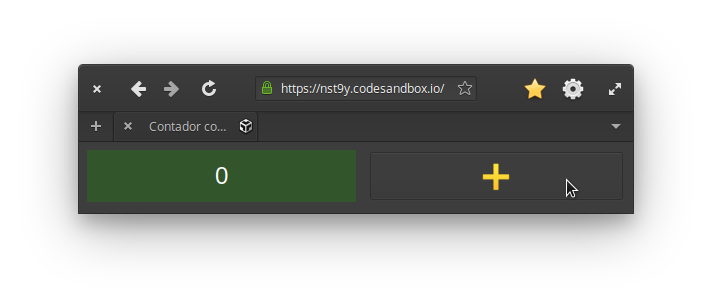
\includegraphics[width=12cm]{./fig/screenshot-contador-epiphany.png}
\end{figure}

A implementação do contador usando classes poder ser observado em
\ref{code:contadorComPOO}.

\begin{listing}[htbp]
\caption{\label{code:contadorComPOO}Contador com POO.}
\begin{minted}[]{js}
// No Java isto extenderia alguma classe padrão do toolkit,
// como `Application`
class Contador {
  constructor(props) {
    // Em Java estas propriedades precisam ser definidas antes
    this.contador = props.valorInicial;
    this.caixaDoValor = document.getElementById("valor");
    this.botãoDeIncrementar = document.getElementById("botãoDeIncrementar");
    this.botãoDeIncrementar.addEventListener(
      "click",
      // Isto requer uma explicação um tanto extensa
      this.tratarClique.bind(this)
    );
  }

  tratarClique(_evento) {
    this.contador = this.contador + 1;
    this.renderizar();
  }

  // Equivalente ao `public static void main()` do Java
  renderizar() {
    this.caixaDoValor.innerText = this.contador;
  }
}

const contador = new Contador({ valorInicial: 0 });
// Como no Java o `main()` é padronizado, sua execução seria
// feita automaticamente pelo ambiente de execução.
contador.renderizar();
\end{minted}
\end{listing}

O \mintinline{js}{tratarClique.bind(this)} na linha 12 requer uma explicação um tanto
extensa.

O contador usando função e operadores do xstream pode ser observado em
\ref{code:contadorComPR}.

\begin{listing}[htbp]
\caption{\label{code:contadorComPR}Contador com PR.}
\begin{minted}[]{js}
import fromEvent from "xstream/extra/fromEvent";

const Contador = props => {
  const caixaDoValor = document.getElementById("valor");
  const botãoDeIncrementar = document.getElementById("botãoDeIncrementar");

  // Fluxo que emite um evento toda vez que o botão for clicado
  const cliqueStream = fromEvent(botãoDeIncrementar, "click");

  // Fluxo que emite "valor + 1" (acumulado) toda vez que
  // cliqueS emite um evento
  const contadorStream = cliqueStream.fold(
    (valor, _evento) => valor + 1,
    props.valorInicial
  );

  const observador = {
    next: valor => {
      caixaDoValor.innerText = valor;
    }
  };

  contadorStream.addListener(observador);
};

Contador({ valorInicial: 0 });
\end{minted}
\end{listing}

\subsubsection{Análise}
\label{sec:org81db0a6}

Essa primeira análise é focada no básico.

\paragraph{Nível de abstração}
\label{sec:org00357e4}
Na solução com POO os conceitos da linguagem que deve-se entender são:
classes, construtor, objetos, propriedades, métodos, \emph{callbacks} na forma
de método, e conhecimento da API do objeto do documento do HTML ---
\emph{Document Object Model (DOM)}.
Além do caso do \mintinline{js}{this} específico do JavaScript:
\mintinline{js}{this.tratarClique.bind(this)}.
Embora sejam conceitos básicos para um programador experiente em JavaScript
e POO, o número é grande.
Abstrações mais sofisticadas não são necessários pelo Contador e o sistema
não insiste em abstrações especiais.
Apesar da solução usar uma quantidade considerável de conceitos, eles são
básicos, então observamos que o Nível de Abstração é baixo, ou seja, bom.

Em contrapartida, na solução com PR os conceitos usados são: funções,
variáveis, fluxos e eventos, callbacks, e a API do DOM.
A abstração mais sofisticada é o método \mintinline{js}{fold()} do fluxo de evento,
que nada mais é que uma versão assíncrona do \mintinline{js}{Array.reduce()}
nativo --- veja a soma de preços em \ref{code:somaDePreçosComReduce}.
Ambos produzem um resultado para cada elemento da lista.
A diferença é que no primeiro a lista é de eventos assíncronos, e infinita.
No segundo a lista é síncrona, com valores escales (números, \emph{strings},
objetos, etc.).
\todo{Paralelo entre métodos assíncronos e síncronos em outra seção?}
Níveis mais altos de abstração não são necessários, então a solução com PR
é igualmente boa ou um pouco melhor que a solução com POO quanto ao Nível
de Abstração.

\paragraph{Proximidade de descrição}
\label{sec:orgc9c6145}
Essa dimensão/critério faz mais sentido para análise de apresentação do que
comportamento (coordenação de eventos).

\paragraph{Dependências ocultas}
\label{sec:orgc129516}
\todo[noline]{Acredito que o HTML só não está situado no mesmo local que o código JavaScript, que é diferente de “oculto”.}
As únicas dependências que podem ser consideradas ocultas são os elementos
HTML buscados pelo identificador com \texttt{document.getElementById("id")}.

\paragraph{Propensão a erros}
\label{sec:org610ef5a}
Na solução com POO, esquecer de vincular a instância do contador à função
\texttt{tratarClique()} resultará no erro “TypeError: this.renderizar is not a
function”.
Pois o valor do \texttt{this} estará vinculado ao objeto que chamou
\texttt{tratarClique()}, ou seja, o \texttt{this.botãoDeIncrementar}.
\todo{Talvez isso seja uma dependência oculta?}
Isso se deve ao fato de a palavra chave \texttt{this} se comportar de forma
diferente no JavaScript quando comparado com outras linguagens.

\begin{citacao}
In most cases, the value of this is determined by how a function is called
(runtime binding). It can't be set by assignment during execution, and it
may be different each time the function is called. ES5 introduced the
bind() method to set the value of a function's this regardless of how it's
called, and ES2015 introduced arrow functions which don't provide their own
this binding (it retains the this value of the enclosing lexical context).
\cite{This2020}.
\end{citacao}

\todo[inline]{Nos próximos exemplos acredito que podemos usar as funções de seta
  como callback no lugar dos métodos, pois possuem o valor do this vinculado
  lexicalmente. O Java possui lambdas desde a versão 8, o que despensa o uso de
  métodos para casos como esse. Ou já removemos desse primeiro? Pra evitar ter
  que explicar o \texttt{.bind(this)} que é um problema específico do
  JavaScript}.

Na solução com PR, esquecer de definir o observador fará com que a
\texttt{caixaDoValor} não seja atualizada.
Pois ela não será renderizada, apesar de toda a lógica do contador
funcionar.
Apesar de tudo, essas possibilidades de erros não são críticas.

\paragraph{Concisão}
\label{sec:org3a4cb87}
Na solução com POO o método \mintinline{js}{tratarClique()}, usado como \emph{callback},
poderia ser substituído por uma função de seta.
Além de poupar algumas linhas o uso do \mintinline{js}{.bind(this)} se torna
desnecessário.
Veja o código do Contador com POO e função de seta em
\ref{code:contadorComPOOeFuncDeSeta} no apêndice.
Na solução com PR a variável intermediária \mintinline{js}{contadorStream} poderia ser
removida, encadeando a chamada do \mintinline{js}{fromEvent} com o \mintinline{js}{fold()}:
\mintinline{js}{const cliqueStream = fromEvent().fold()}.
No entanto essa manobra diminuiria a legibilidade do
código\footnote{Note que o nome da variável \mintinline{js}{cliqueStream} já nem faz mais
sentido, pois o resultado da expressão não inclui apenas os eventos de clique.}.
De qualquer forma, a PR evita a verbosidade da declaração da classe e dos
métodos, além da repetição do \mintinline{js}{this}.
Então em termos de Concisão a PR está à frente da POO.

\paragraph{Viscosidade}
\label{sec:orgcb6d0e7}
Num caso tão simples como o do Contador a única resistência a alteração
está em renomear atributos no caso da POO, e variáveis na PR.
No entanto isso é inevitável ao renomear termos.
Além disso o IDE pode ajudar através de uma funcionalidade de refatoração.
\todo{Talves seja interessante analisar a viscosidade da alteração pra colocar um botão de decremento (-1) do Contador.}

\subsection{Reserva de voo}
\label{sec:org0b7dd7a}
